
\chapter{Analysis}

\section{Introduction}

\subsection{Client Identification}
My client, Shahida Rahman, is an Author, and the Director and Secretary of Perfect Publishers Ltd, which has been a self publishing company since 2005. This means that the author pays Perfect Publishers to publish their book. She published her first book through Perfect Publishers Ltd, and this was when the company was born. She is 42 years old and is a mother of 4 children. Shahida uses computers to deal with online enquiries and to publish books from all over the world. Furthermore, she also produces the royalty statements for each book twice yearly. Aside from this, she has little experience with computers. Shahida generally uses a computer for research, social networking and reading the news. Every book is outsourced to an Editor and a Cover Designer. When the book is fully edited and formatted to the right specifications, they return the ready to print files to Shahida, who sends the books off to print. They track the books and their details manually using a database on an Excel Spreadsheet. Currently, it is difficult to keep all the data up to date and it is rather disorganised. Shahida would like to be able to look up a book/number of books in the system by using the details, such as the Author/Title/Date etc. She would also like the new system to link this database with information about the royalties of each book, and when they are needed to be paid every six months. The system could send an email to her, updating her about these.

\subsection{Define the current system}
The system that is currently being used consists of Shahida entering the book and its details into the spreadsheet. These details are taken from the enquiries that she receives via email, and include; first name, last name, email, and vague details of the book. Then, the more accurate details such as; book title, size, number of pages, hardback/paperback, mat or gloss, crème or white paper, font and font size are discussed between Shahida and the customer. She also records their details in a separate spreadsheet, which includes their email, phone number, and address, upon the customer's consent. The spreadsheets are used to track current and previous customers and their books, as the details about the book and themselves are recorded in these. Subsequently, Shahida informs the customer of the price details, waits for full payment and  then sends the customer an invoice. She then contacts her editor and her illustrator to start work on the book. Shahida refers to her company's website, where the calculated prices are ready for books, in order to correctly price the book, in accordance to the book’s details. An ISBN number is assigned to the book, which is bought in bulks by Shahida from the ISBN Office. Once the book is finished, the book is sent off to print, and the author receives 25 copies.

\subsection{Describe the problems}
There are numerous problems with the current system. First of all, the usage of the spreadsheet makes it harder to find a customer and their details, and their book’s details. This is because the spreadsheet is much disorganised. Furthermore, it is harder to keep track of the details of each book, meaning it is difficult to update the details of the book when necessary. Because there are a large number of books in the system, it is harder to find each book and then seperately find the customer that the book was written by, as they are in seperate spreadsheets, meaning that Shahida must manually search for them in both spreadsheets. Also, if the same author makes an enquiry about another book, their details must be entered into the spreadsheet again, because it is difficult to find where the customers details currently are due to there being many customers in the spreadsheet, having incorrectly entered their data from a given enquiry, or they might have been removed after having been there for a long time This could cause inconsistencies in the data, because for instance, the customer may move house, meaning their address would need changing, and it would be difficult to find and update all entries where their address is recorded. 
\subsection{Section appendix}

\begin{figure}[H]
    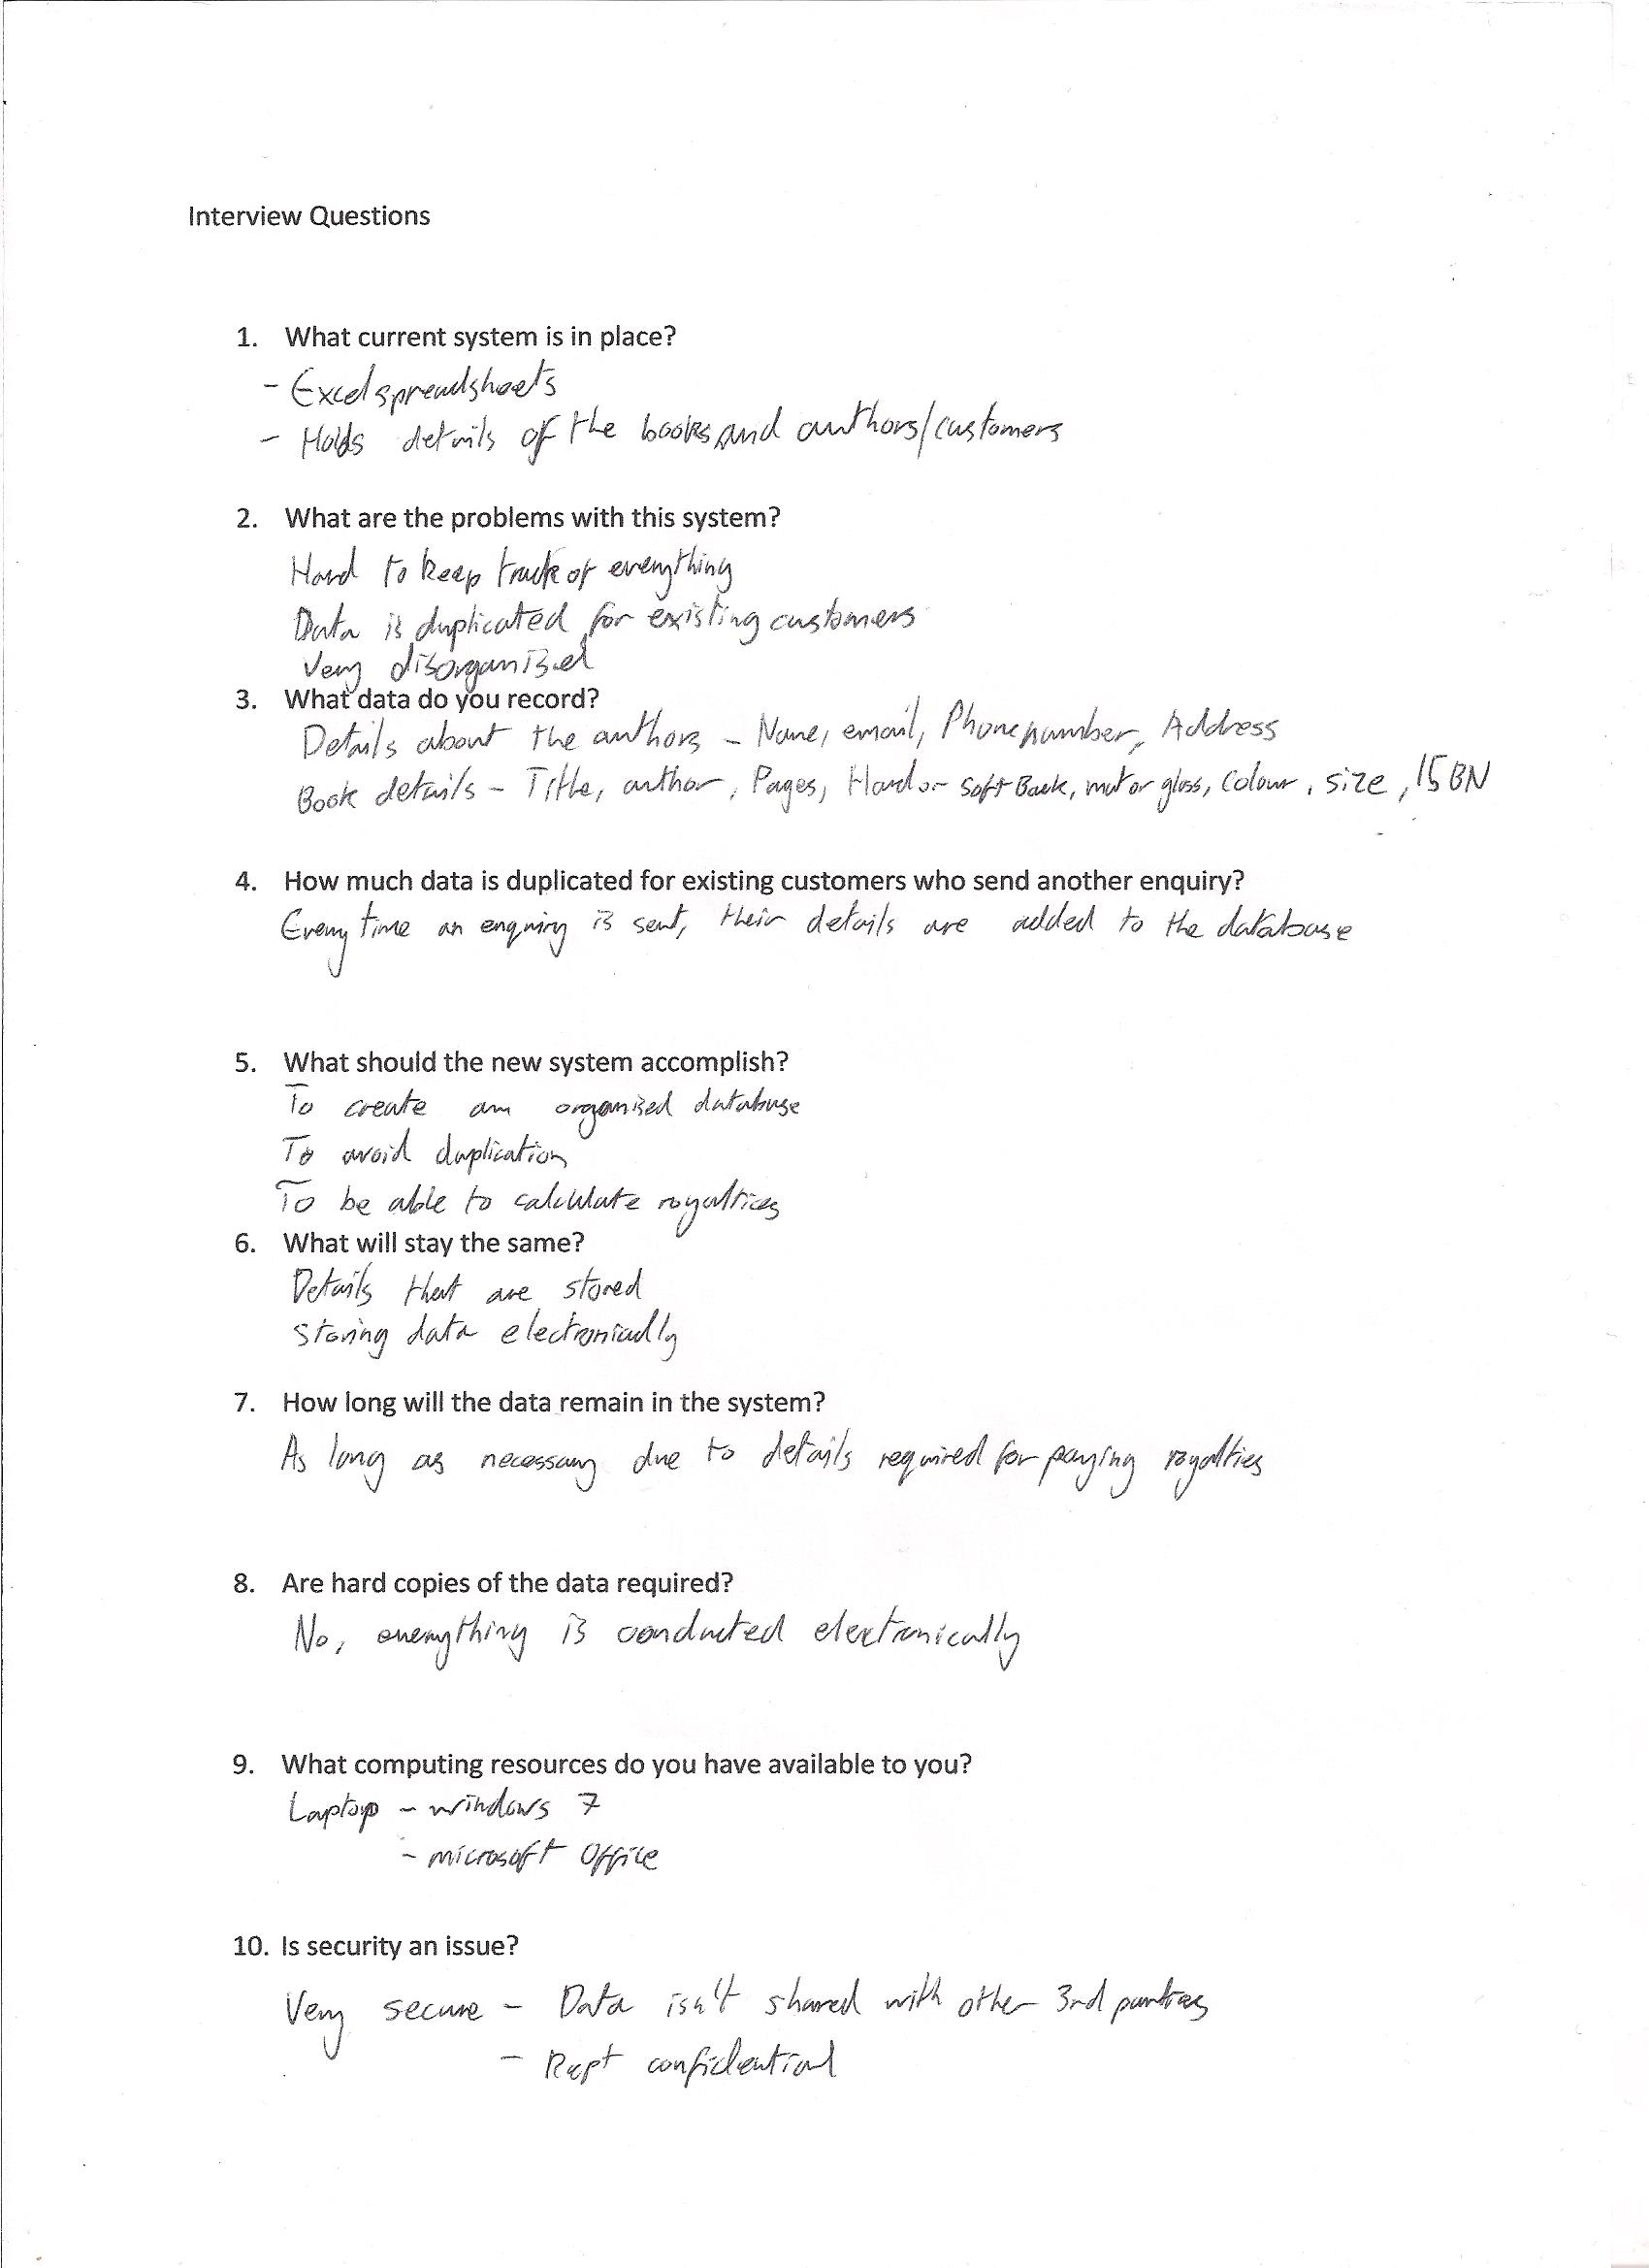
\includegraphics[width= 10cm]{./Analysis/Interview_Questions_1.jpg}
    \caption{Interview Questions: Page 1} \label{Interview_Questions_1.jpg}
\end{figure}

\begin{figure}[H]
    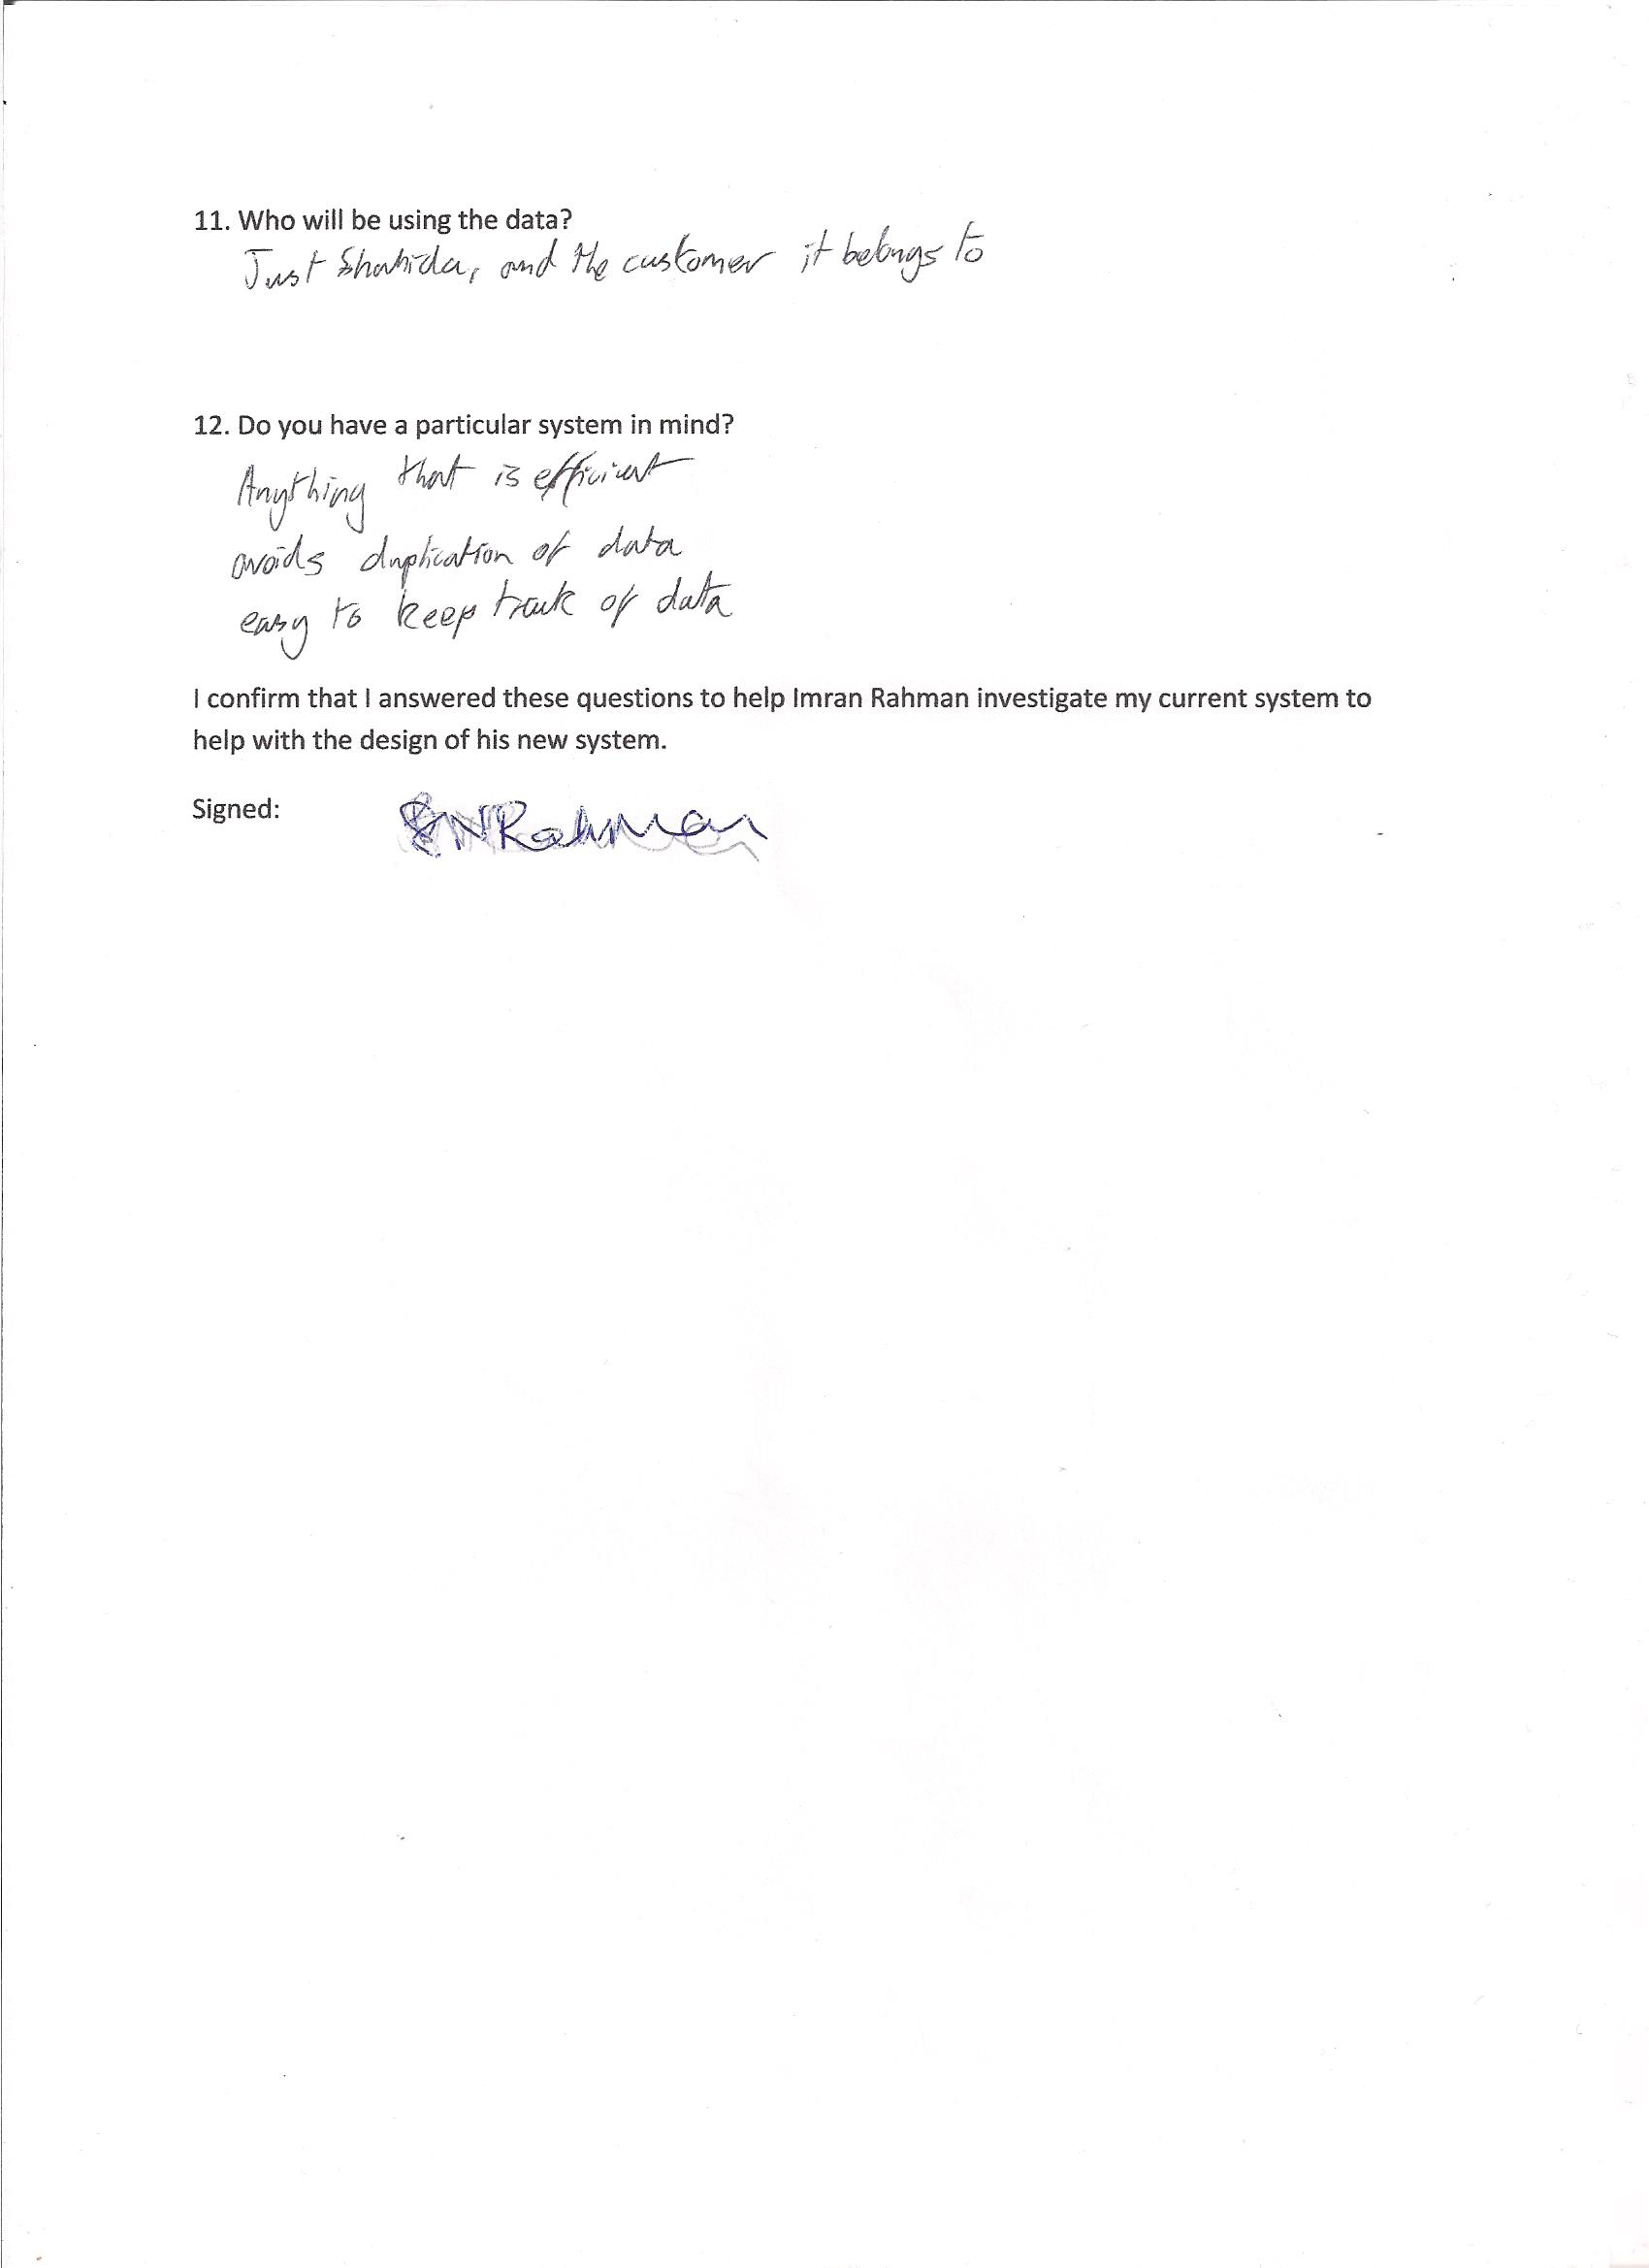
\includegraphics[width=\textwidth]{./Analysis/Interview_Questions_2.jpg}
    \caption{Interview Questions: Page 2} \label{Interview_Questions_2.jpg}
\end{figure}

\section{Investigation}

\subsection{The current system}

\subsubsection{Data sources and destinations}
In the current system there are three key data sources that are used. These are Shahida herself, the customer and the spreadsheets. The Customer sends the enquiry which is sent via email. After the details about the book have been discussed, they are stored in one spreadsheet, and the details of the customer are stored in a seperate spreadsheet, linked to the details of the book. These details are agreed seperately from the enquiry, between Shahida and the customer. Details such as the book size, page number, hardback/softback and paper type are used to calculate the cost for the customer, which is used to create an invoice which is sent to the customer. This is the first output of the system. A copy of every invoice is stored on Shahida's computer in a special folder just for invoices. Once Shahida receives full payment, the work is conducted and completed. If the customer wishes to publish another book, they send another enquiry, and their personal data is duplicated because of the details of the new book which are added. Every six months after the book has been published, the royalties must be paid to the author. The royalties are the profit that the author makes from sales of her book from bookshops. A royalty statement is created and stored in a special folder just for royalties.

\begin{center}
\begin{tabular}{|p{3.5cm}|p{3.5cm}|p{3cm}|p{3cm}|}
    \hline
    \textbf{Source} & \textbf{Data} & \textbf{Example Data} & \textbf{Destination} \\ \hline
    Customer Enquiry & Forename & Peter & Shahida  \\ \hline
    Customer Enquiry & Surname & Parker & Shahida  \\ \hline
    Customer Enquiry & Email & mail@example.com & Shahida  \\ \hline
    Customer & Address & 1 Example Road & Shahida  \\ \hline
    Customer & Postcode & AB1 2CD & Shahida  \\ \hline
    Customer & Phone Number & 07123456789 & Shahida  \\ \hline
    Customer & Book Title & The Hobbit & Shahida \\  \hline
    Customer & Size & Large & Shahida \\  \hline
    Customer & Number of Pages & 395 & Shahida \\  \hline
    Customer & Hardback/Paperback & Paperback & Shahida \\  \hline
    Customer & Mat/Gloss & Gloss & Book Database \\  \hline
    Customer & Creme/White Paper & White Paper & Shahida \\  \hline
    Customer & Font & Times New Roman & Shahida \\  \hline
    Customer & Font Size & 12 & Shahida \\  \hline
    Shahida & Book Title & The Hobbit & Book Database \\  \hline
    Shahida & Size & Large & Book Database \\  \hline
    Shahida & Number of Pages & 395 & Book Database \\  \hline
    Shahida & Hardback/Paperback & Paperback & Book Database \\  \hline
    Shahida & Mat/Gloss & Gloss & Book Database \\  \hline
    Shahida & Creme/White Paper & White Paper & Book Database \\  \hline
    Shahida & Font & Times New Roman & Book Database \\  \hline
    Shahida & Font Size & 12 & Book Database \\  \hline
    Shahida & Forename & Peter & Author Database  \\ \hline
    Shahida & Surname & Parker & Author Database  \\ \hline
    Shahida & Email & mail@example.com & Author Database  \\ \hline
    Shahida & Address & 1 Example Road & Author Database  \\ \hline
    Shahida & Postcode & AB1 2CD & Author Database  \\ \hline
    Shahida & PhoneNumber & 07123456789 & Author Database  \\ \hline
    Shahida & Invoice & - & Invoice Folder \\ \hline
    Shahida & Invoice & - & Customer  \\ \hline
    Shahida & ISBN & 9780007525492 & Book Database \\ \hline
    Shahida & Date Published & 23/10/2014 & Book Database \\ \hline
    Shahida & Price & £12.99 & Book Database \\ \hline
    Customer & Payment & £1000 & Shahida  \\ \hline
    Shahida & Cover Preferences & - & Cover Designer\\ \hline
    Shahida & Book & - & Editor  \\ \hline
    Editor & Completed Book & - & Shahida  \\ \hline
    Cover Designer & Completed Cover & - & Shahida \\ \hline
    Shahida & Royalty Statement & - & Royalty Statement Folder \\ \hline
    Shahida & Royalty Statement & - & Customer \\ \hline
    Shahida & Royalties & £211.20 & Customer \\ \hline 
    \hline
\end{tabular}
\end{center}


\subsubsection{Algorithms}
In the current system there are two Algorithms which are being used. The first sends an invoice to the customer and checks whether Shahida has recieved full payment. Once Shahida has received full payment, she, her cover designer and her editor can begin working on the book. The second algorithm consists of completing the work that is needed to be done, and checks whether the work has been completed, so that the completed book can then be sent off for printing. 

\begin{algorithm}[H]
    \caption{First Algorithm - Sending an invoice and Checking for Payment}
\begin{algorithmic}[1]

\SET{$Payment$}{$false$}
\State

Check Website for Price

Create Invoice

Send Invoice

\While{$Payment = false$}

     Check For Payment

     \If{$Payment Received$}

     	Payment = true

     \EndIf
\EndWhile
\end{algorithmic}
\end{algorithm}


\begin{algorithm}[H]
    \caption{Second Algorithm - Completing Work and Checking If Work is Completed}
\begin{algorithmic}[1]
\SET{$WorkComplete$}{$false$}
\SET{$CoverComplete$}{$false$}
\SET{$BookComplete$}{$false$}
\State

\While{$WorkComplete = false$}
    
    Get Completed Cover from Cover Designer

    \SET{$CoverComplete$}{$true$}

    Get Completed Book from Editor

    \SET{$BookComplete$}{$true$}

    \If{$BookComplete \ and \ CoverComplete$}

        \SET{$finished$}{$true$}

    \EndIf
\EndWhile
\end{algorithmic}
\end{algorithm}

\subsubsection{Data flow diagrams}

\begin{figure}[H]
    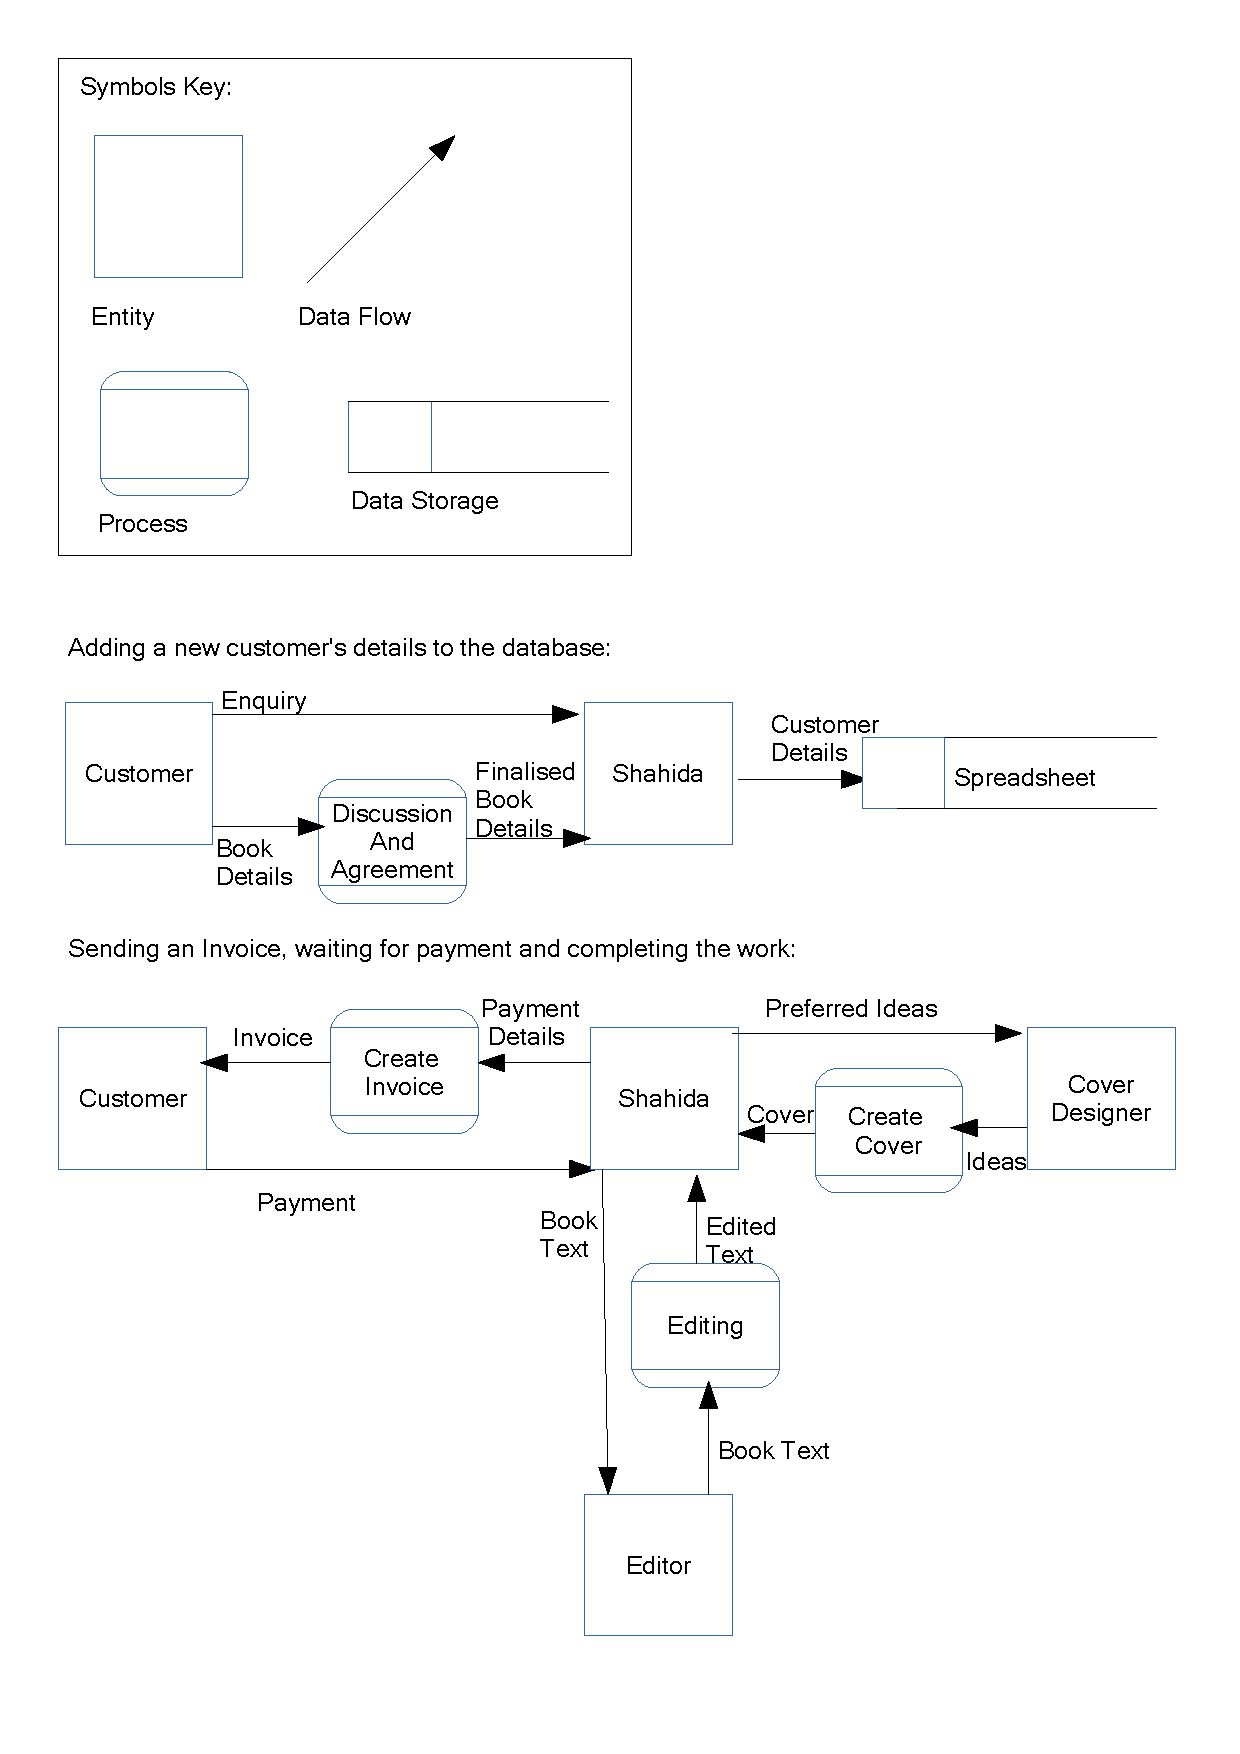
\includegraphics[width=\textwidth]{./Analysis/Data_Flow_Diagrams_1.pdf}
    \caption{Data Flow Diagrams} \label{Data_Flow_Diagrams_1.pdf}
\end{figure}

\subsubsection{Input Forms, Output Forms, Report Formats}

The current system has just one input form. This is the Enquiry that is sent to the company, from an author. Also, The current system has two different output forms - The Invoice and The Royalty Statement.


The enquiry is received via email, which is sent using the company's website. The email will look like this when received:


First Name:

Last Name:

Email:

Question/Comment:



The following image is an example of the first output form, an Invoice.

\begin{figure}[H]
    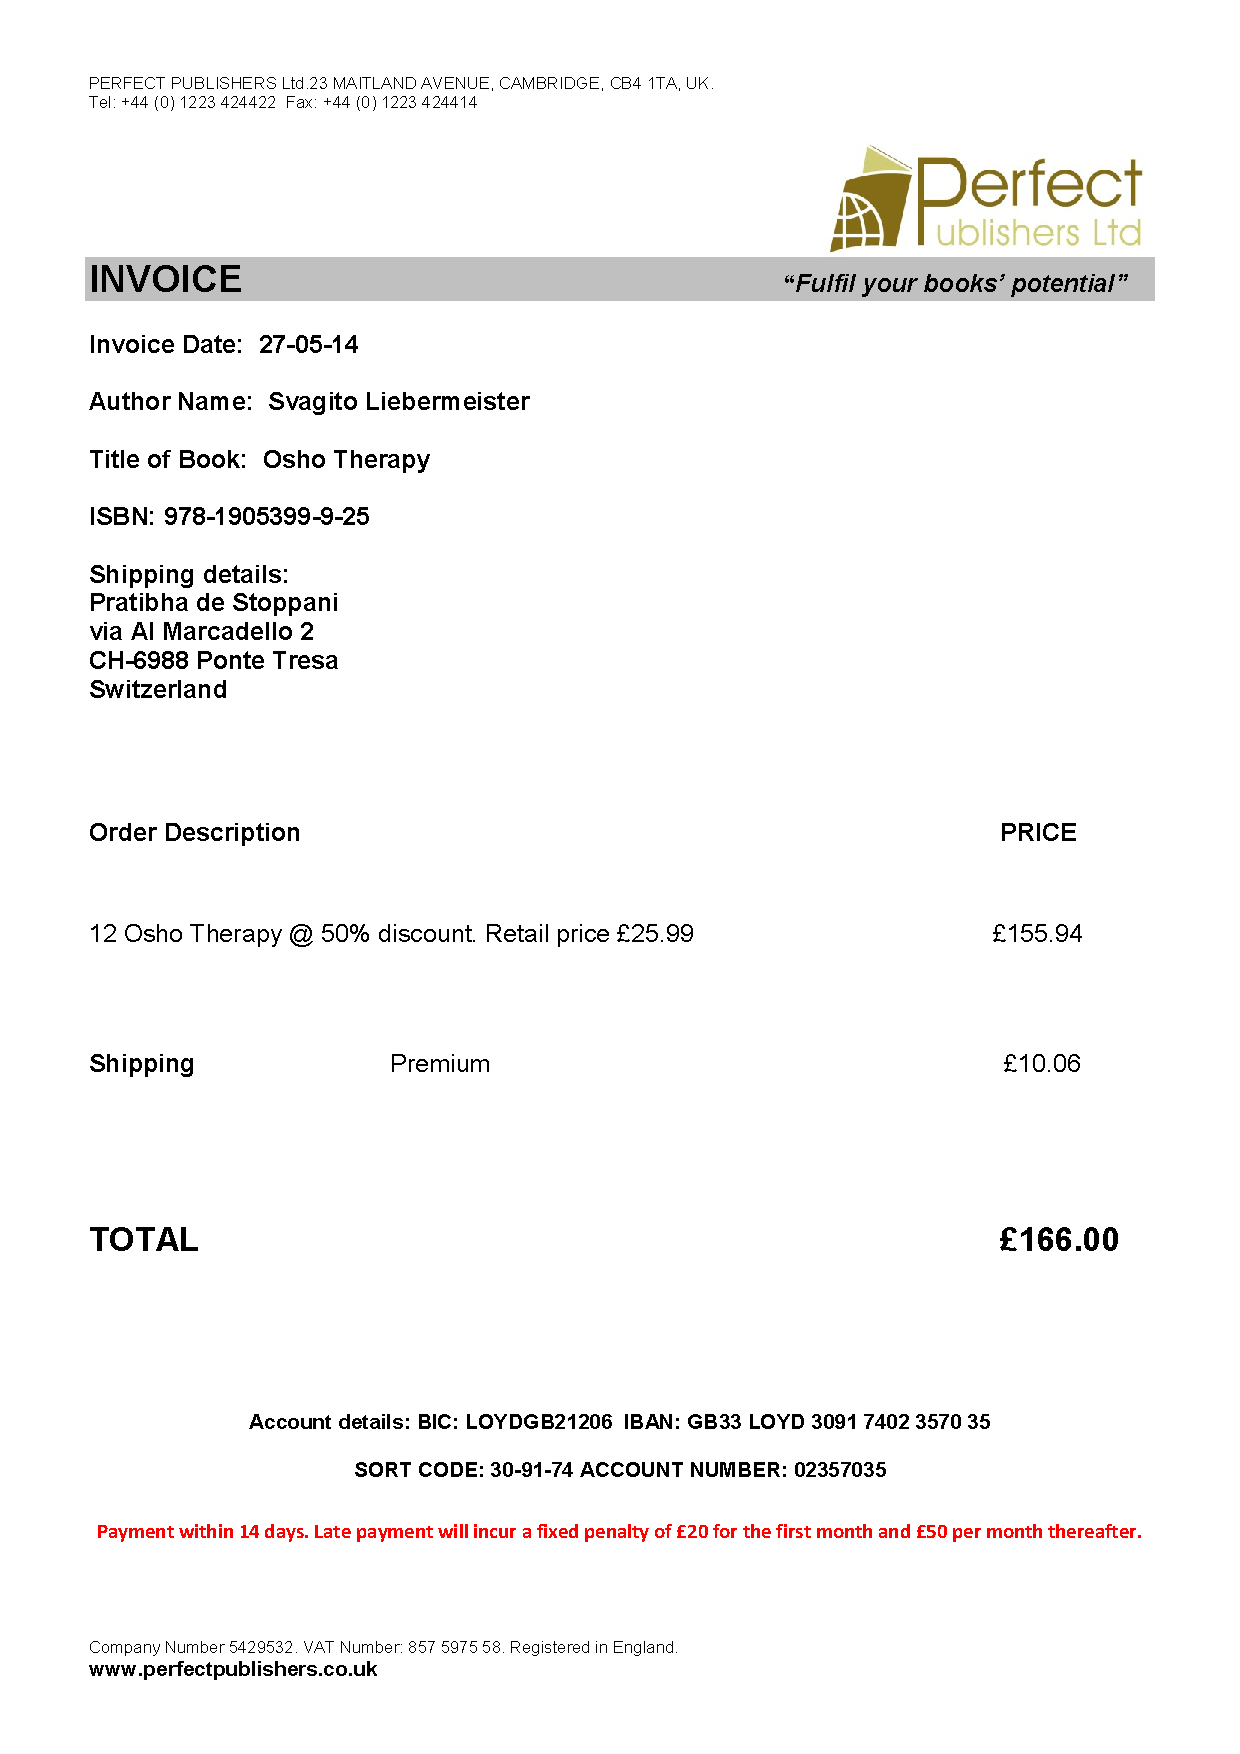
\includegraphics[width=\textwidth]{./Analysis/Invoice_Example.pdf}
    \caption{Invoice Example} \label{Invoice_Example.pdf}
\end{figure}


The following image is an example of the second output form, a Royalty Statement.

\begin{figure}[H]
    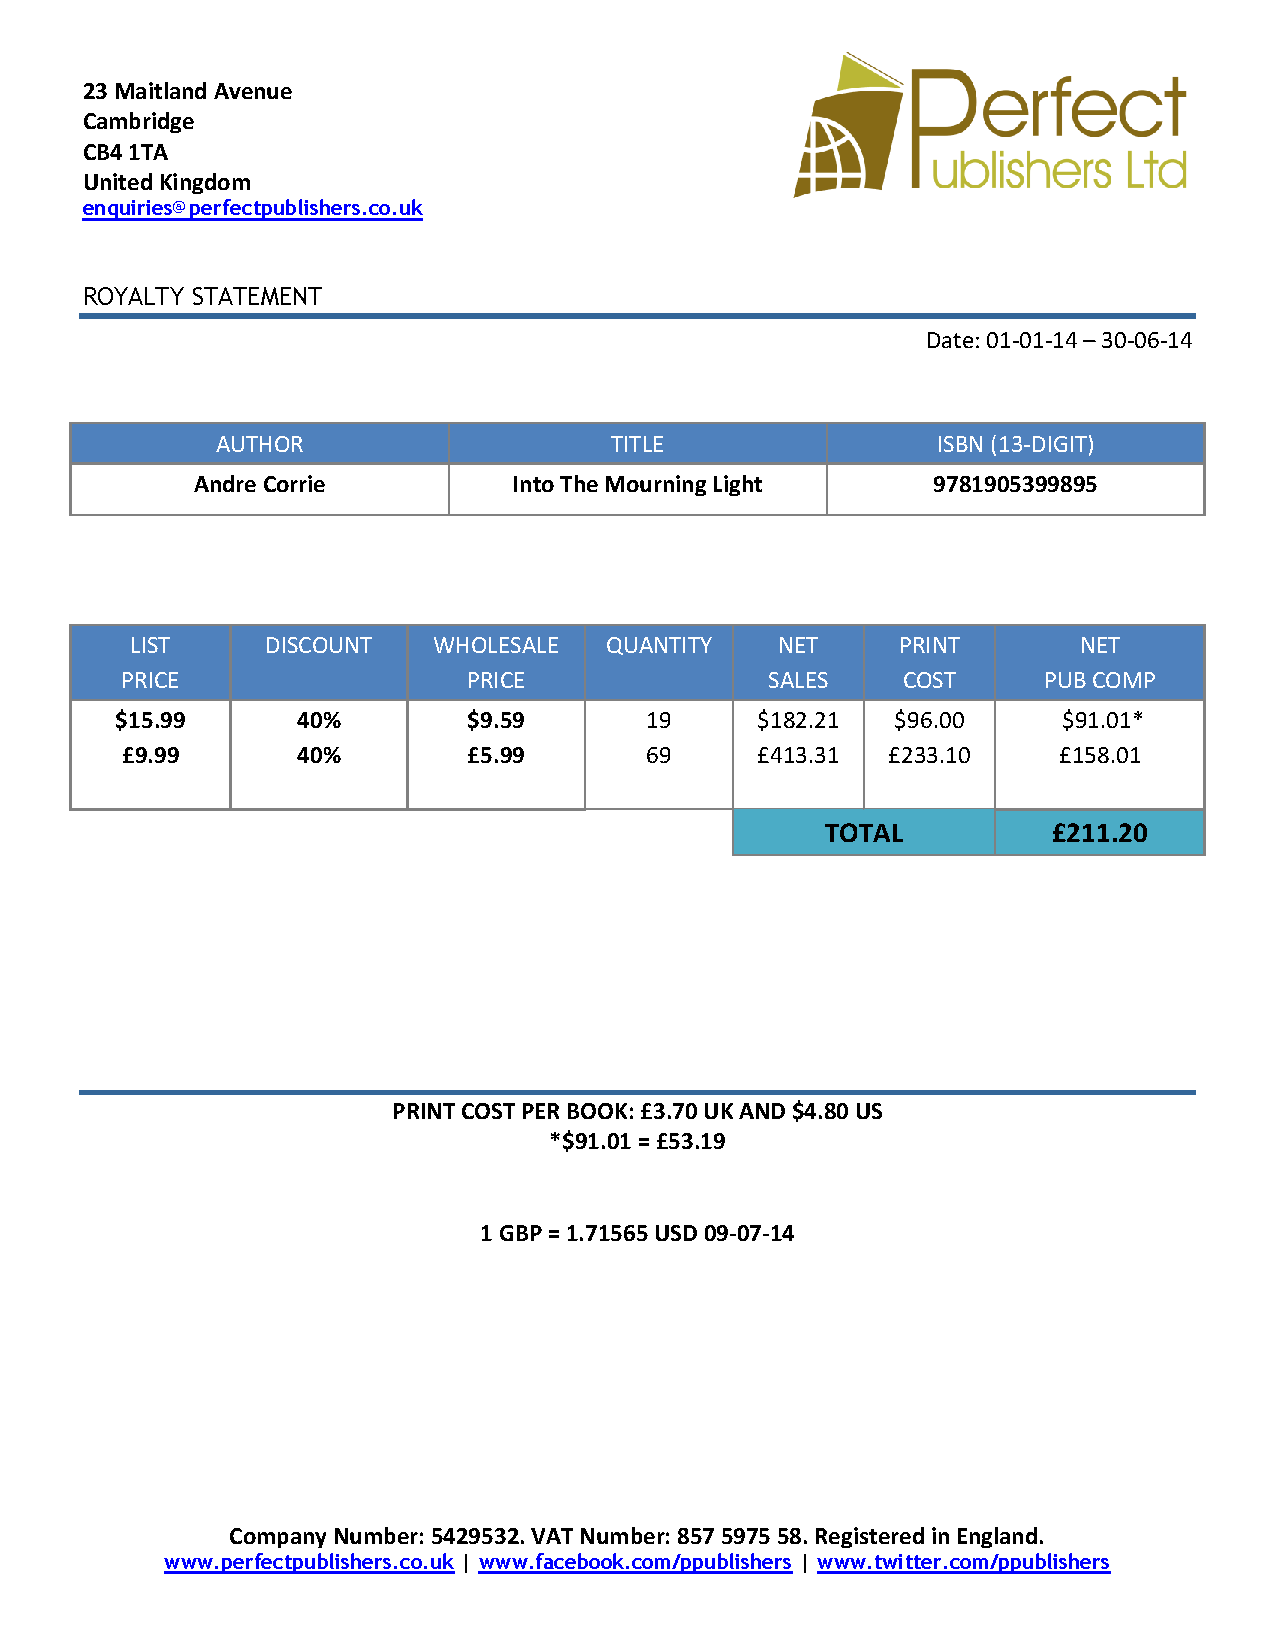
\includegraphics[width=\textwidth]{./Analysis/Royalty_Statement_Example.pdf}
    \caption{Royalty Statement Example} \label{Royalty_Statement_Example.pdf}
\end{figure}

\subsection{The proposed system}

In the proposed system the Customer's information will still be received through the online form on the company's website, which Shahida receives via email. She will then enter this into the system using a new interface that will ask her for the details. This will be placed into a database. Each Customer's book will have a primary key, the ISBN number which Shahida assigns to the book. In a seperate database, the author's details will be stored and the author will have a special ID number which is used only in the databases. Every book that is published by the same author will have an attribute which is the author's ID. The ID will just be a number. The system's interface will have a search feature, which can search for book titles, authors, and author IDs.

\subsubsection{Data sources and destinations}
\begin{center}
\begin{tabular}{|p{3cm}|p{3.5cm}|p{3cm}|p{2.5cm}|}
    \hline
    \textbf{Source} & \textbf{Data} & \textbf{Data Type} & \textbf{Destination} \\ \hline
    Customer Enquiry & Forename & String & Shahida  \\ \hline
    Customer Enquiry & Surname & String & Shahida  \\ \hline
    Customer Enquiry & Email & String & Shahida  \\ \hline
    Customer & Address & String & Shahida  \\ \hline
    Customer & Postcode & String & Shahida  \\ \hline
    Customer & Phone Number & String & Shahida  \\ \hline
    Customer & Book Title & String & Shahida \\  \hline
    Customer & Size & String & Shahida \\  \hline
    Customer & Number of Pages & 395 & Shahida \\  \hline
    Customer & Hardback/Paperback & Paperback & Shahida \\  \hline
    Customer & Mat/Gloss & Gloss & Shahida \\  \hline
    Customer & Creme/White Paper & White Paper & Shahida \\  \hline
    Customer & Font & Times New Roman & Shahida \\  \hline
    Customer & Font Size & 12 & Shahida \\  \hline
    Shahida & Book Title & The Hobbit & Database \\  \hline
    Shahida & Size & Large & Database \\  \hline
    Shahida & Number of Pages & 395 & Database \\  \hline
    Shahida & Hardback/Paperback & Paperback & Database \\  \hline
    Shahida & Mat/Gloss & Gloss & Database \\  \hline
    Shahida & Creme/White Paper & White Paper & Database \\  \hline
    Shahida & Font & Times New Roman & Database \\  \hline
    Shahida & Font Size & 12 & Database \\  \hline
    Shahida & Forename & String & Database  \\ \hline
    Shahida & Surname & String & Database  \\ \hline
    Shahida & Email & String & Database  \\ \hline
    Shahida & Address & String & Database  \\ \hline
    Shahida & Postcode & String & Database  \\ \hline
    Shahida & PhoneNumber & String & Database  \\ \hline
    Shahida & ISBN & String & Database \\ \hline
    Shahida & Date Published & Date & Database \\ \hline
    Shahida & Price & Real & Book Database \\ \hline
    Database* & Author ID & Integer & Shahida  \\ \hline
    Shahida & Invoice & String & Invoice Folder \\ \hline 
    Shahida & Invoice & String & Customer  \\ \hline
    Customer & Payment & Real & Shahida  \\ \hline
    Shahida & Cover Details & String & Cover Designer\\ \hline
    Shahida & Book & String & Editor  \\ \hline
    Editor & Completed Book & String & Shahida  \\ \hline
    Cover Designer & Completed Cover & Image & Shahida \\ \hline
    Shahida & DatePublished & Date & Database \\ \hline 
    Shahida & Royalty Statement & - & Royalty Statement Folder \\ \hline
    Shahida & Royalty Statement & - & Customer \\ \hline
    Shahida & Royalties & Real & Customer \\ \hline 
	
    \hline
\end{tabular}
\end{center}
*The Database will create a number and assign that number as an Author ID

\subsubsection{Data flow diagram}

\begin{figure}[H]
    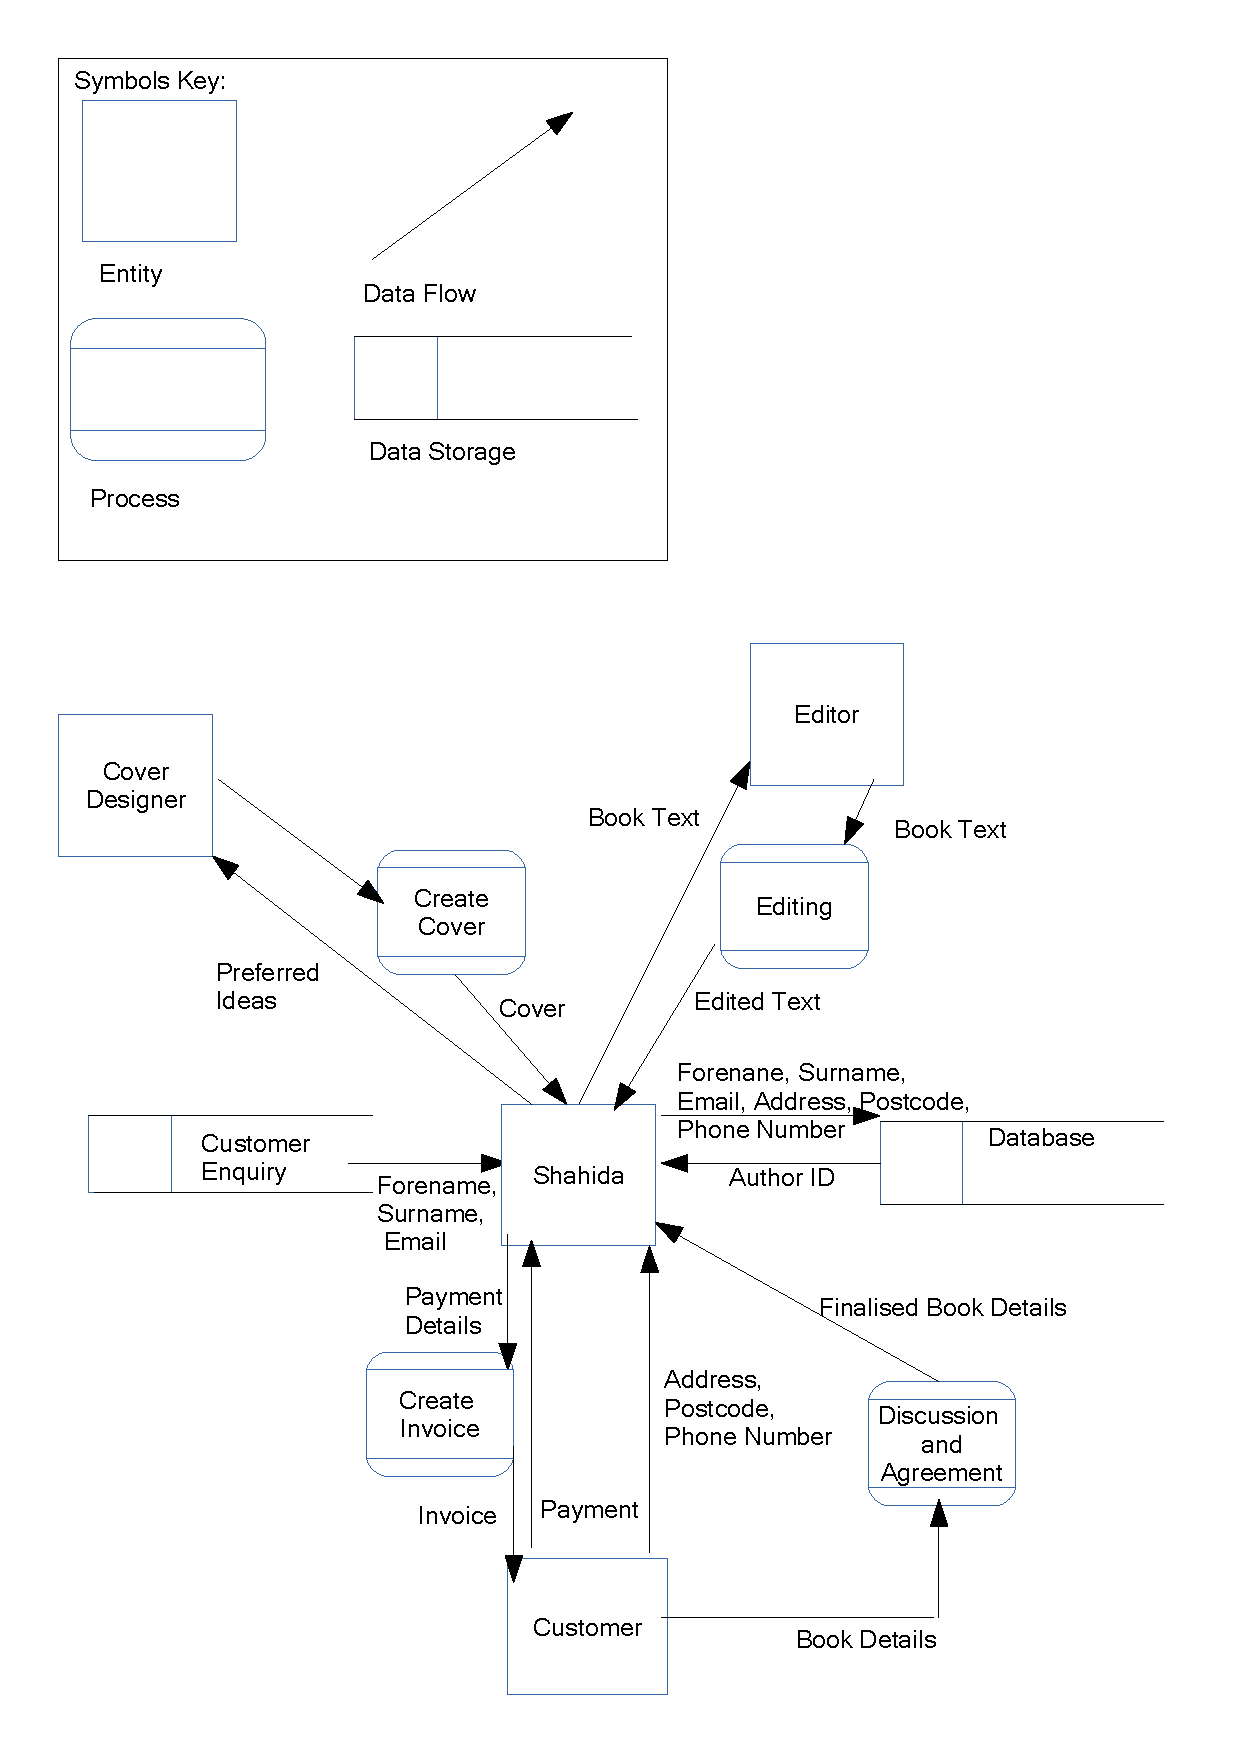
\includegraphics[width=\textwidth]{./Analysis/Data_Flow_Diagrams_2.pdf}
    \caption{Data Flow Diagram} \label{Data_Flow_Diagrams_2.pdf}
\end{figure}

\subsubsection{Data dictionary}

\begin{center}
\begin{tabular}{|p{2.5cm}|p{1.5cm}|p{2.5cm}|p{2.5cm}|p{3.5cm}|}
    \hline
    \textbf{Name} & \textbf{Data Type} & \textbf{Length} & \textbf{Validation} & \textbf{Example Data} \\ \hline
    FirstName & String & 2-20 Characters & Length & Jo  \\ \hline
    LastName & String & 2-20 Characters & Length & Williamson  \\ \hline
    Email & String & 7-30 Characters & Length & mail@example.com  \\ \hline
    PhoneNumber & String & 9-15 Characters & Format & 07123456789  \\ \hline
    Address & String & 5-64 Characters & Length & Example Road  \\ \hline
    Postcode & String & 7 Characters & Format & AB1 2CD  \\ \hline
    Author ID & Integer & 1-255 & Range & 17  \\ \hline
    ISBN & String & 13 Characters & Length & 9780007525492 \\ \hline
    BookTitle & String & 1-127 Characters & Length & The Hobbit  \\ \hline
    NoOfPages & Integer & 1-1023 & Range & 395  \\ \hline
    Size & String & 5 & Existence & Large \\ \hline
    Back & String & 8 or 9 Characters& Existence & Paperback  \\ \hline
    Cover & String & 3 or 5 Characters & Existence & Gloss \\ \hline
    Paper & String & 11 Characters & Existence & White Paper\\ \hline
    Font & String & 1-64 Characters & Length & Arial  \\ \hline
    FontSize & Real & 8-64 & Numbers only & 12.5  \\ \hline
    DatePublished & Date & dd/mm/yyyy & Range & 23/10/2014 \\ \hline
    Price & Real & Numbers only & £12.99 \\ \hline
    \hline
\end{tabular}
\end{center}

\subsubsection{Volumetrics}

I have conducted calculations to calculate the maximum  possible size of 1 customer and book record, which is 275 Bytes. However, when a customer wishes to publish more than one book, more book records are required. As the most amount of books one customer has published with the company is 3, we can have 4 book records per customer record.

Each ASCII Character is 1 byte, each number up to 255 is 1 byte, and each number between 256 and 32768 is 2 bytes. Real Numbers such as 12.5 are 2 bytes, and a Date is 3 bytes.

Firstly, I have worked out the size of the customer record, which is 157 Bytes.

FirstName (20) + LastName (20) + Email (30) + PhoneNumber (15) + Address (64) + Postcode (7) + Author ID (1) = 157 Bytes.

I have then calculated the size of one book record, which is 118 Bytes.
Book Title (1), NoOfPages (2), Size (5), Back (9), Cover (5), Paper (11), Font (64), FontSize (2) + ISBN (13) + DatePublished (3) + Price (2) + Author ID (1) = 118 Bytes

If we have 4 book records per customer record, that would mean that the size for 1 customer with 4 books would be 157 + (5 * 118) = 747 Bytes.

I have chosen to use a size of 100 different customer records, which would be equivalent to 74700 bytes, and 74700 / 1024 = 72.9 Kilobytes. This is because the company rarely have more than 20 enquiries in a year. This would be a suitable number of customer records as it will last a few years before it may require resizing, which can be conducted at a later date when necessary. 72.9 KB will be not be difficult for Shahida's PC to hold, as it is a very small size.

\section{Objectives}

\subsection{General Objectives}

The general objectives are:
\begin{itemize}
    \item Organised layout for the database.
    \item Prevention of unnecessary duplication of data.
    \item Simple interface for entering data, meaning it can be conducted quickly.
    \item Search function to find a specific customer in the database.
    \item Ability to edit existing data easily and quickly.
\end{itemize}

The System must be able to prevent unecessary duplication of data, and be able to organise data well, and this will be a priority.

\subsection{Specific Objectives}

Organising a new layout for the database:

\begin{itemize}
    \item Be able to sort by date (ascending and descending)
    \item Clear tables and fields for each entity and attribute
\end{itemize}


Preventing Duplication:

\begin{itemize}
    \item Checks to see if the data already exists
    \item Use of Author ID to ensure it will only be entered once
\end{itemize}


Simple interface for entering data:

\begin{itemize}
    \item As little amount of boxes as possible
    \item Clearly label entry boxes
\end{itemize}


Search function and editing data:

\begin{itemize}
    \item Data can be found using the Author ID, Author Name, or Book Title
    \item Can be edited upon finding the desired data
\end{itemize}

\subsection{Core Objectives}

\begin{itemize}
    \item Organising the data using certain attributes
    \item Preventing Duplication
\end{itemize}

\subsection{Other Objectives}

\begin{itemize}
    \item Searching for data using attributes
    \item Editing data in the database
\end{itemize}

\section{ER Diagrams and Descriptions}

\subsection{ER Diagram}

\begin{figure}[H]
    \caption{ER Diagram} \label{ER_Diagram.pdf}
    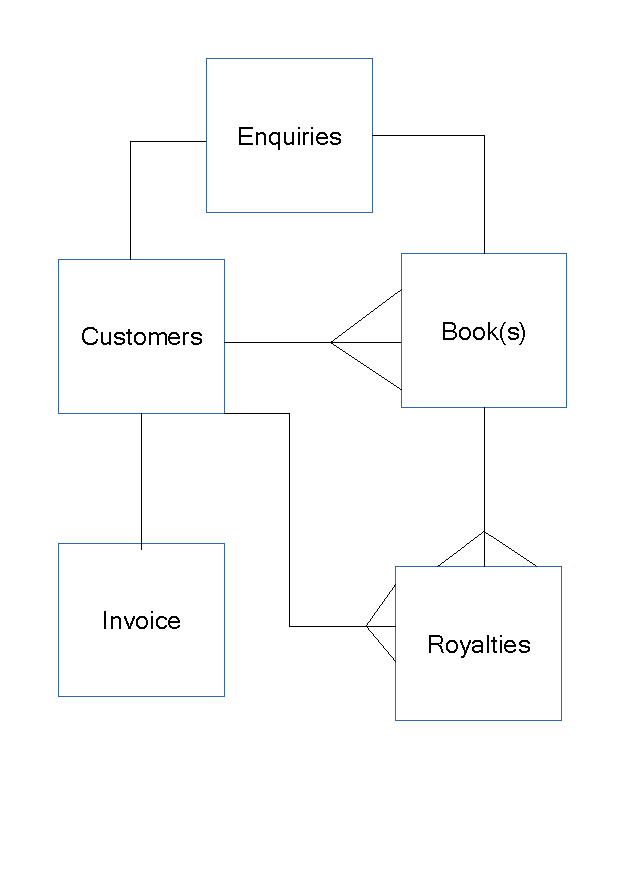
\includegraphics[width=\textwidth]{./Analysis/ER_Diagram.pdf}
\end{figure}

\subsection{Entity Descriptions}

Customer(\underline{Author ID}, \emph{Email}, Forename, Surname, Address, Postcode, Phone Number)

Enquiry(\underline{Email}, \emph{Author ID}, Forename, Surname)

Invoice(\underline{Author ID}, \emph{ISBN Number}, Book title, Price, Forename, Surname, Address, Postcode)

Royalties(\underline{AuthorID}, \emph{ISBN Number}, Book title, Price, Forename, Surname, Address, Postcode)

Book(\underline{ISBN Number}, \emph{AuthorID}, Book Title, Pages, Size, Cover type, Colour, Back Type, Paper, Font, Font size, Date published, Price)

The database will only store data about the customers and their books, as the enquiries give details about the books and customers, and the royalties and invoices are stored seperately from the database.

\section{Object Analysis}

\subsection{Object Listing}

\begin{itemize}
    \item Shahida
    \item Customer
    \item Editor
    \item Cover Designer
    \item Spreadsheet

\end{itemize}

\subsection{Relationship diagrams}

\begin{figure}[H]
    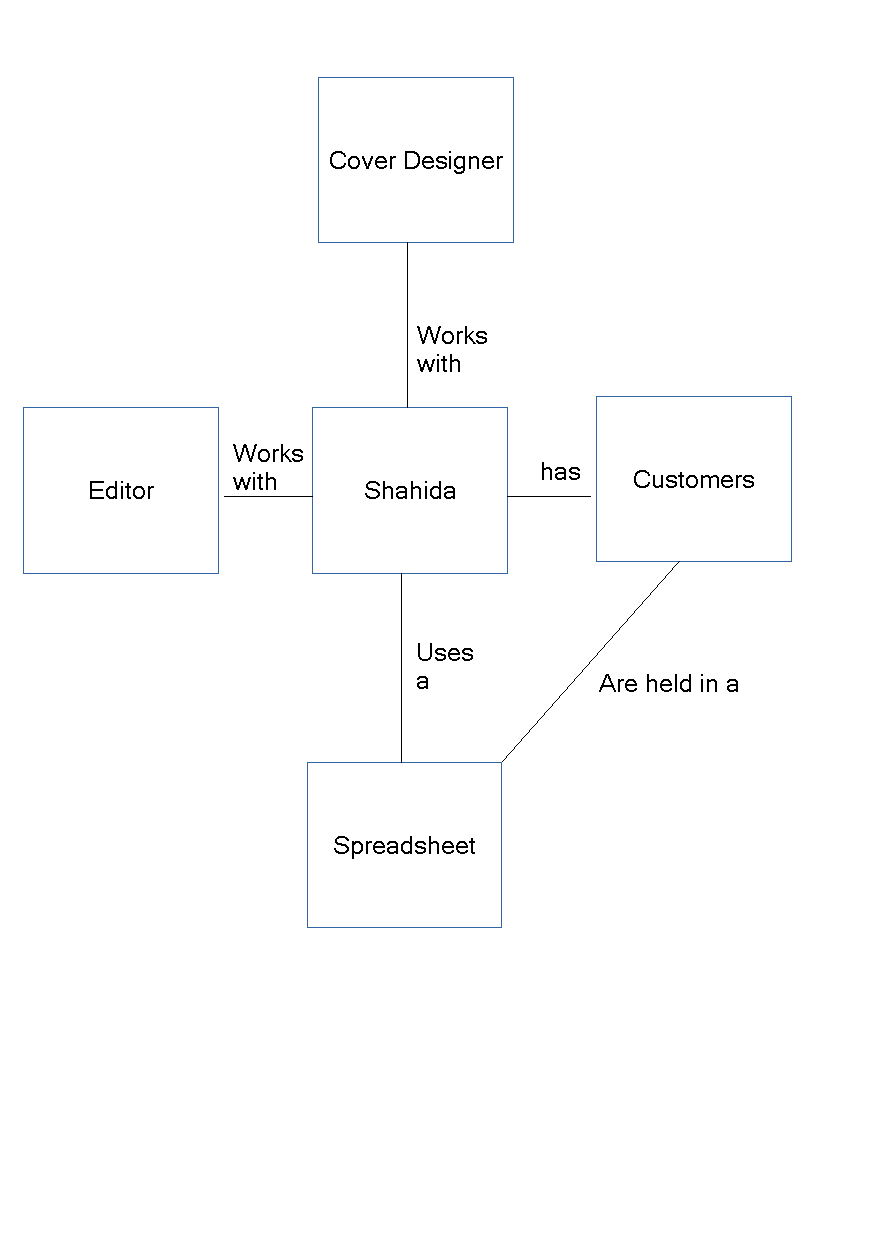
\includegraphics[width=\textwidth]{./Analysis/Relationship_Diagram.pdf}
    \caption{Relationship Diagram} \label{Relationship_Diagram.pdf}
\end{figure}

\subsection{Class definitions}

Key:

\begin{tabular}{|p{2.5cm}|}
    \hline
    \textbf{Label}  \\ \hline
    Attributes \\ \hline
    Behaviours  \\ \hline
    \hline
\end{tabular}

\begin{tabular}{|p{2.5cm}|}
    \hline
    \textbf{Customer} \\ \hline
    Author ID \\ ForeName \\ Surname \\ Email \\ Address \\ Postcode \\ Phone Number \\ \hline
    Add ForeName \\ Edit Forename \\ Add Surname \\ Edit Surname \\ Add Email \\ Edit Email \\ Add Address \\ Edit Address \\ Add Postcode \\ Edit Address \\ Add Postcode \\ Edit Postcode \\ Add Phone Number \\ Edit Phone Number \\ \hline
    \hline
\end{tabular}

\begin{tabular}{|p{2.5cm}|}
    \hline
    \textbf{Book} \\ \hline
    Title \\ ISBN \\ Pages \\ Size \\ Cover Type \\ Colour \\ Back Type \\ Paper \\ Font \\ Font Size \\ \hline
    Add Title \\ Edit Title \\ Add ISBN \\ Edit ISBN \\ Add Pages \\ Edit Pages \\ Add Size \\ Edit Size \\ Add Cover Type \\ Edit Cover Type \\ Add Colour \\ Edit Colour \\ Add Back Type \\ Edit Back Type \\ Add Paper \\ Edit Paper \\ Add Font \\ Edit Font \\ Add Font Size \\ Edit Font Size\\ Add Date Published \\ Edit Date Published \\ Add Price \\ Edit Price \\ \hline
    \hline
\end{tabular}

\section{Other Abstractions and Graphs}
Graphs not required.

\section{Constraints}

\subsection{Hardware}
Shahida uses her laptop to run the company from home. The new system will need to be able to run on this machine.

Computer Specifications:

\begin{itemize}
    \item 15.6” Display
    \item AMD Quad-Core A4-5000M APU (1.5GHz, 2MB cache)
    \item 4 GB DDR3 RAM
    \item 750 GB HDD, 5400 rpm
    \item AMD Radeon HD 8330 Graphics Card
\end{itemize}

The proposed system will have no problem with running on this machine, as it uses a small amount of CPU usage. A constraint would be the size of the screen. This is because the system will need to be based around the screen size of her laptop. As her laptop is portable, portability is not a constraint. The laptop will need enough RAM to hold the system. However, Shahida's laptop has more than enough memory for this, meaning this will not be a problem. 

\subsection{Software}

Shahida would prefer that the system will run on Windows 7, as she uses this operating system for her laptop. Changing the operating system will cause difficulties, meaning it is best for the system to run on Windows 7, suiting her needs.

\subsection{Time}

Shahida does not need this system to be built quickly, but she would like it to be complete as soon as reasonably possible. Otherwise, the only deadline for this project is April 2015, which has been set by my teacher.

\subsection{User Knowledge}

Having worked in the publishing industry beforehand, being an author has also given Shahida the knowledge of how to run her current company. Aside from being able to perform basic tasks on a computer, browsing the internet and using social media, Shahida has small experience with computers.

\subsection{Access restrictions}

Shahida will be the only person who will have full access to all the data in the proposed system, and she will be the only one who can access it. This can be password protected for security reasons, meaning that only she can gain access to the database. This is also because she is the only necessary person to view, enter and edit data in the system, as her Editor and her Cover Designer do not need to use the database. As she is the only user of the database, it will be easier to keep secure. The authors will be able to make requests about personal data, such as having it removed, or receiving a copy of the personal data about them. The database will comply to the Data Protection Act 1998, as the company already does so with their current system.

\section{Limitations}

\subsection{Areas which will not be included in computerisation}
Generally, all actions require the use of a computer in the company. However, rarely, a customer does call Shahida about an enquiry, as this customer may not be so computer literate. In this case, Shahida will note down the details of the enquiry, and will enter it into the database.

\subsection{Areas considered for future computerisation}

The database could be used online, so that the authors can use their Author ID to log in and see just their details on the database. This would mean that the customers would not have to contact Shahida to receive the data held about them, as they can see the data by theirselves. They will also be able to access this data from anywhere where they have access to the internet. This could also enable Shahida to access the data from other machines aside from her laptop.

\section{Solutions}

\subsection{Alternative solutions}
\begin{center}
\begin{tabular}{|p{2.5cm}|p{3.5cm}|p{3.5cm}|}
    \hline
    \textbf{Solution} & \textbf{Advantages} & \textbf{Disadvantages} \\ \hline

    Re-organisation of the current spreadsheet & No changes to current operating system and software required, will not cost & Current problems will still occur, Difficult to keep organised as it will require more maintenance to do so \\ \hline

    Python Desktop Application with GUI & User Friendly, Clear and easy to interpret, Layout can be designed specificly for the client, Usage of buttons simplifies tasks, Minimal training needed for most levels of experience & Takes up more memory, Takes longer to create the application  \\ \hline

    Filing system & No electronics needed, Costs less, Minimal training needed for most levels of experience & Difficult to back up the data due to it being held on paper, data will have to be sent via post when necessary, Lots of physical space is required, more prone to damage and deteriation due to more movement \\ \hline

    \hline
\end{tabular}
\end{center}
\subsection{Justification of chosen solution}
I have chosen to use the Python Desktop Application with GUI as my solution. This is because:

\begin{itemize}
    \item I am already familiar with the Python Programming Language, whereas I have little knowledge of how to manage a Paper Filing system or with creating advance spreadsheets.
    \item This will keep the system using computers and software, meaning there will not be a drastic change.
    \item Using the application will take less time than manually entering everything into a spreadsheet.
    \item This will also take less time and physical space than writing details down on paper.
\end{itemize}
